\documentclass[11pt,aspectratio=169]{beamer}

\usepackage{slides}
\usepackage{soul}
\usepackage{pdfpc}
\usepackage{ebproof}
\usepackage{bigdelim}
\usepackage{booktabs}
\usepackage{listings}
\usepackage{tcolorbox}
\usepackage{tabularx}
\usepackage{tikz}
\usepackage{xspace}
\usepackage[T1]{fontenc}
\usepackage[utf8]{inputenc}
\usepackage[symbol]{footmisc}
\usepackage[noend]{algpseudocode}
\usepackage[
    backend    = biber,
    style      = alphabetic,
    giveninits = true,
    maxnames   = 16,
    minnames   = 16,
]{biblatex}

\addbibresource{./references.bib}

\usetikzlibrary{
    positioning,
    shapes.symbols,
    shadows,
    arrows,
    calc
}

\newcommand{\senc}{\text{senc}}
\newcommand{\msg}{\text{msg}}
\newcommand{\nonce}{\text{nonce}}
\newcommand{\KDF}{\text{KDF}}
\newcommand{\key}{\text{key}}

\newcommand{\Tamarin}[1]{\textsc{Tamarin}\xspace}

%% Print: [#1] -[#2]-> [#3]
\newcommand{\MSR}[3]{#1 -\hspace{-4pt}[\hspace{5pt} #2 \hspace{4pt}]\hspace{-4.6pt}\rightarrow #3}
%% Print: -[#1]->
\newcommand{\ActionFact}[1]{-\hspace{-4pt}[\hspace{5pt} #1 \hspace{4pt}]\hspace{-4.6pt}\rightarrow}
%% Print: ~
\newcommand{\tildelow}{\raisebox{0.5ex}{\texttildelow}}
%% Print: ^
\newcommand{\pow}{\textasciicircum{}}
%% Highlight text in overlay
\newcommand{\althl}[2][2]{\alt<#1>{\hl{#2}}{#2}}

%% Sticky notes to represent facts
\definecolor{StickyNoteYellow}{RGB}{241,239,161}
\definecolor{StickyNoteRed}{RGB}{255,167,169}
\definecolor{StickyNoteGreen}{RGB}{148,199,146}
\definecolor{StickyNoteBlue}{RGB}{167,229,241}
\NewDocumentCommand{\StickyNote}{O{StickyNoteYellow}O{1cm}m}{%
    \begin{tikzpicture}
        \node[
            drop shadow={
                shadow xshift = 2pt,
                shadow yshift = -4pt,
            },
            xslant = -0.1,
            yslant = 0.1,
            draw   = black,
            fill   = #1,
            text   = black,
        ] {\parbox[t][#2][c]{#2}{\centering#3}};
    \end{tikzpicture}
}

%% Colors for terms and facts
\definecolor{TermBlue}{HTML}{1C377D}
\definecolor{FactPurple}{HTML}{7C3655}

\newcommand{\term}[1]{\textcolor{TermBlue}{#1}}
\newcommand{\Term}[1]{\textcolor{TermBlue}{#1}}
\newcommand{\Fact}[1]{\textcolor{FactPurple}{#1}}

%% Other colors
\definecolor{AdversaryRed}{HTML}{DA3B26}

%% Listings
\lstset{escapeinside={(*@}{@*)}}
\lstset{numberstyle=\tiny}

\definecolor{TamarinBlue}{RGB}{42,0,255}
\definecolor{TamarinGreen}{RGB}{48,110,32}
\definecolor{TamarinPurple}{RGB}{175,36,67}

\lstdefinestyle{tamarin}{
    basicstyle    = \linespread{0.75}\footnotesize\ttfamily,
    extendedchars = true,
    tabsize       = 2,
    columns       = fixed,
    numbers       = none,
    breaklines    = true,
    literate      = {~}{{\raisebox{0.5ex}{\texttildelow}}}{1},
    morekeywords  = {theory, builtins, restriction, equations, functions, rule,
                     let, in, lemma, All, Ex, not, predicates, begin, end},
    keywordstyle  = \color{TamarinPurple},
    morecomment   = [l]{//},
    morecomment   = [s]{/*}{*/},
    commentstyle  = \color{TamarinGreen},
    xleftmargin   = 0mm,
    upquote       = true,
    morestring    = *[b]",
    showstringspaces = false
}

\lstdefinestyle{tactic}{
    basicstyle    = \linespread{0.75}\footnotesize\ttfamily,
    extendedchars = true,
    tabsize       = 2,
    columns       = fixed,
    numbers       = none,
    breaklines    = true,
    literate      = {~}{{\raisebox{0.5ex}{\texttildelow}}}{1},
    alsoletter    = :,
    morekeywords  = {tactic:, presort:, prio:, deprio:},
    keywordstyle  = \color{TamarinPurple},
    morecomment   = [l]{//},
    morecomment   = [s]{/*}{*/},
    commentstyle  = \color{TamarinGreen},
    xleftmargin   = 0mm,
    upquote       = true,
    morestring    = *[b]",
}

\lstdefinestyle{oracle}{
    basicstyle    = \linespread{0.75}\footnotesize\ttfamily,
    extendedchars = true,
    tabsize       = 2,
    columns       = fixed,
    numbers       = none,
    breaklines    = true,
    literate      = {~}{{\raisebox{0.5ex}{\texttildelow}}}{1},
    morecomment   = [l]{\#},
    morekeywords  = {import, for, in, if, elif},
    keywordstyle  = \color{TamarinPurple},
    commentstyle  = \color{TamarinGreen},
    xleftmargin   = 0mm,
    upquote       = true,
}

\definecolor{ProVerifGreen}{RGB}{48,110,32}
\definecolor{ProVerifBlue}{RGB}{64,112,161}

\lstdefinestyle{proverif}{
    basicstyle    = \linespread{0.75}\footnotesize\ttfamily,
    extendedchars = true,
    tabsize       = 2,
    columns       = fixed,
    numbers       = none,
    breaklines    = true,
    literate      = {~}{{\raisebox{0.5ex}{\texttildelow}}}{1},
    morecomment   = [s]{(*}{*)},
    commentstyle  = \color{ProVerifGreen},
    keywordstyle  = \color{ProVerifBlue},
    morekeywords  = {in, if, event, new, let, out},
    xleftmargin   = 0mm,
}

\definecolor{proofTreeBlue}{HTML}{2639B0}
\definecolor{proofTreeRed}{HTML}{921C12}

\lstdefinestyle{prooftree}{
    basicstyle    = \linespread{0.8}\footnotesize\fontfamily{pcr}\selectfont,
    extendedchars = true,
    tabsize       = 2,
    columns       = fixed,
    numbers       = left,
    breaklines    = true,
    literate      = {~}{{\raisebox{0.5ex}{\texttildelow}}}{1},
    keywords      = [1]{lemma, case, next, qed, by, end, Diff-Lemmas},
    keywordstyle  = [1]\color{black}\bfseries,
    keywords      = [2]{simplify, solve, sorry, contradiction, induction,
                        autoprove, rule-equivalence},
    keywordstyle  = [2]\color{proofTreeBlue}\bfseries,
    keywords      = [3]{@, \|, <, \^},
    keywordstyle  = [3]\color{proofTreeRed},
    alsoletter    = @\|<\^-,
    moredelim     = **[is][{\color{proofTreeBlue}}]{<<}{>>},
    xleftmargin   = 0mm,
    upquote       = true,
    morestring    = *[b]",
}

%% Color boxes
\definecolor{ColorBoxBlue}{HTML}{1C377D}
\tcbset{
    colback      = white,
    colframe     = black,
    fonttitle    = \bfseries,
    coltitle     = white,
    colbacktitle = ColorBoxBlue,
    boxrule      = 1pt
}

%% Vertical separator for frames
\newcommand<>{\vsep}{
    \begin{tikzpicture}[remember picture,overlay]%
        \draw[ultra thick]
            ($(current page.north west)+(8cm,0.5cm)$) to
            ($(current page.south west)+(8cm,-0.5cm)$)
        ;
    \end{tikzpicture}%
}

%% Horizontal separator for frames
\newcommand<>{\hsep}{
    \begin{tikzpicture}[remember picture,overlay]%
        \draw[ultra thick]
            ($(current page.north west)+(-0.5cm,-4.5cm)$) to
            ($(current page.north east)+(0.5cm,-4.5cm)$)
        ;
    \end{tikzpicture}%
}


\title{Formal Analysis of Real-World Security Protocols}
\subtitle{Lecture 4: Verification Theory (Part 1)}
\date{\today}
\author{Aleksi Peltonen}
\institute{CISPA Helmholtz Center for Information Security}

\begin{document}
\maketitle

% ---------------------------------------------------------------------------- %
% Content
% ---------------------------------------------------------------------------- %

\begin{frame}[fragile]{This lecture}
    \tableofcontents
\end{frame}

% ---------------------------------------------------------------------------- %

\section{Tamarin Workflow}

% ---------------------------------------------------------------------------- %

\begin{frame}[fragile]{The Tamarin prover}
    \begin{tikzpicture}[remember picture, overlay]
        \node[left, yshift=.5cm] (img) at (current page.center) {
            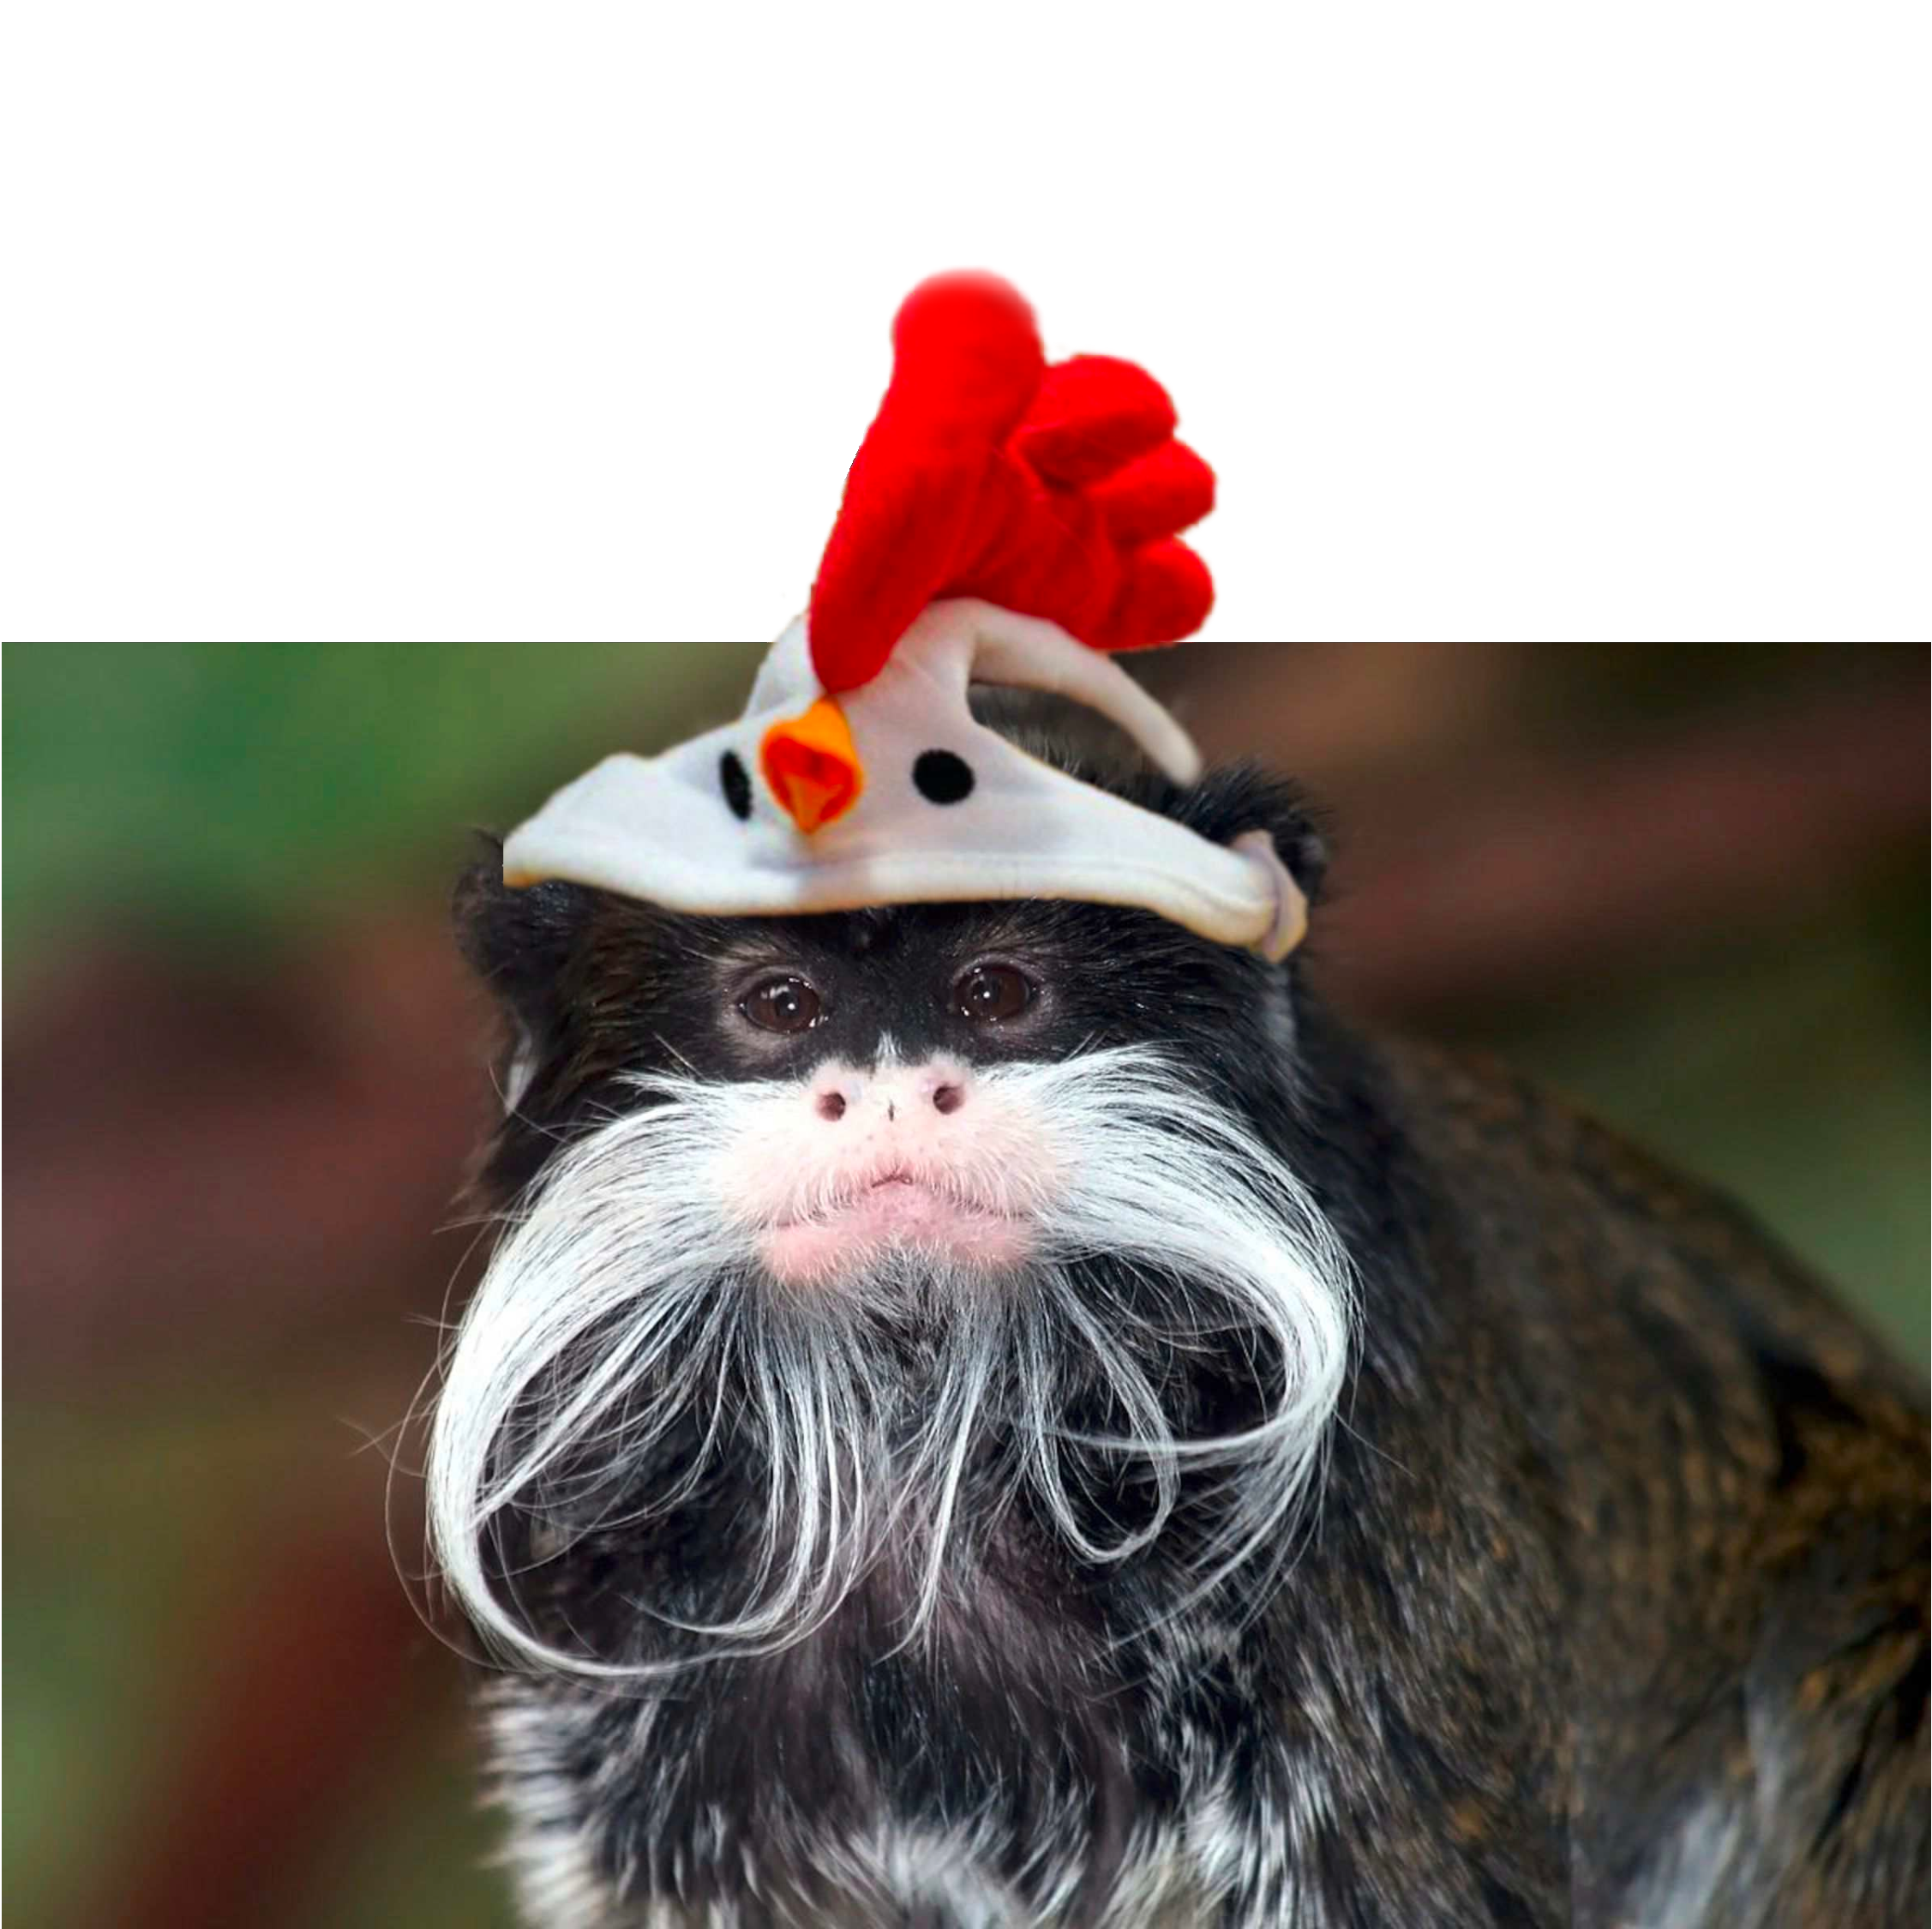
\includegraphics[width=0.4\textwidth]
                {./figures/lecture_0/tamarin_photo_hat}
        };
        \draw[
            line width=1mm,
            triangle 45-,
            color=orange,
        ] (img.east) +(0,-1.8) -- +(2,-1.8) node[right] {Constraint solver};
        \draw[
            line width=1mm,
            triangle 45-,
            color=orange,
        ] (img.east) +(0,-.3) -- +(2,-.3) node[right] {Theorem prover};
    \end{tikzpicture}
\end{frame}

\begin{frame}[fragile]{Tamarin workflow}
    \begin{figure}
        \includegraphics<1>[width=.8\textwidth]
            {./figures/lecture_4/tamarin_workflow_1}%
        \includegraphics<2>[width=.8\textwidth]
            {./figures/lecture_4/tamarin_workflow_2}%
        \includegraphics<3>[width=.8\textwidth]
            {./figures/lecture_4/tamarin_workflow_3}%
        \includegraphics<4>[width=.8\textwidth]
            {./figures/lecture_4/tamarin_workflow_4}%
        \includegraphics<5>[width=.8\textwidth]
            {./figures/lecture_4/tamarin_workflow_5}%
        \includegraphics<6>[width=.8\textwidth]
            {./figures/lecture_4/tamarin_workflow_6}%
        \includegraphics<7>[width=.8\textwidth]
            {./figures/lecture_4/tamarin_workflow_7}%
        \includegraphics<8>[width=.8\textwidth]
            {./figures/lecture_4/tamarin_workflow_8}%
    \end{figure}
\end{frame}

\begin{frame}[fragile]{Semantics}
    \begin{itemize}
        \item \textbf{Transition relation}
        \begin{itemize}
            \item[] $S\,\ActionFact{a}_R\,(( S \smallsetminus^{\#} l )
                    \cup^{\#} r)$, where
            \begin{itemize}
                \item $\MSR{l}{a}{r}$ is a ground instance of a rule in $R$, and
                \item $l\subseteq^{\#}S$ wrt the equational theory
            \end{itemize}
        \end{itemize}
        \item \textbf{Executions}
        \begin{itemize}
            \item $execs(R) = \{\;[\;]\,\ActionFact{a_1} \dots \ActionFact{a_n}
                  \, S_n \;|\; \forall n .\; Fr(n)$ appears only once on the 
                  right-hand side of the rule\;\}
        \end{itemize}
        \item \textbf{Traces}
        \begin{itemize}
            \item $traces(R) = \{\; [a_1, \dots , a_n] \;|\; [\;]\,\ActionFact
                  {a_1} \dots \ActionFact{a_n}\, S_n \in execs(R)\;\}$
        \end{itemize}
        \item \textbf{Question:} Can we reach a specific state
              (encoded by actions)?
    \end{itemize}
\end{frame}

\begin{frame}[fragile]{Example}
    \begin{table}[]
        \footnotesize
        \begin{tabular}{ll}
            MSR & Alternative syntax \\
            \toprule
            \begin{lstlisting}[style=tamarin, gobble=16]
                rule r1:
                    [ Fr(~a), Fr(~k) ]
                    -->
                    [ St(~a, ~k)
                    , Out(enc(~a,~k))
                    , Key(~k) ]
            \end{lstlisting} &
            $\mathrm{\dfrac{Fr(a)\quad Fr(k)}{St(a,k)\quad
            Out(enc(a,k))\quad Key(k)}}$ \\
            \midrule
            \begin{lstlisting}[style=tamarin, gobble=16]
                rule r2:
                    [ St(a, k)
                    , In(<a, a>) ]
                  --[ Fin(a, k) ]->
                    [ ]
            \end{lstlisting} &
            $\mathrm{\dfrac{St(a,k)\quad In(\langle a,a \rangle)}{}[Fin(a,k)]}$ 
            \\
            \midrule
            \begin{lstlisting}[style=tamarin, gobble=16]
                rule r3:
                    [ Key(k) ]
                  --[ Rev(k) ]->
                    [ Out(k) ]
            \end{lstlisting} &
            $\mathrm{\dfrac{Key(k)}{Out(k)}[Rev(k)]}$ \\
            \bottomrule \\
            \begin{lstlisting}[style=tamarin, gobble=16]
                // Fin(a, k) is reachable
                lemma trace: exists-trace
                    " Ex a k #i . Fin(a, k)@i "
            \end{lstlisting} &
            $\exists a,k (Fin(a,k))$
        \end{tabular}
    \end{table}
\end{frame}

\begin{frame}[fragile]{Example}
    \begin{table}[]
        \tiny
        \vspace*{-.5cm}
        \begin{tabular}{rl}
            \textbf{MSR Instances} & \textbf{Resulting State} \\
            \toprule
            $\mathrm{\dfrac{}{Fr(a)}}$
                & \{Fr(a)\}$^{\sharp}$ \\
            \midrule
            $\mathrm{\dfrac{}{Fr(k)}}$
                & \{Fr(a), Fr(k)\}$^{\sharp}$ \\
            \midrule
            $\mathrm{\dfrac{Fr(a)\quad Fr(k)}{St(a,k)\quad Out(enc(a,k))\quad Key(k)}}$
                & \{St(a,k), Out(enc(a,k)), Key(k)\}$^{\sharp}$ \\
            \midrule
            $\mathrm{\dfrac{Key(k)}{Out(k)}[Rev(k)]}$
                & \{St(a,k), Out(enc(a,k)), Out(k)\}$^{\sharp}$ \\
            \midrule
            $\mathrm{\dfrac{Out(k)}{K(k)}}$
                & \{St(a,k), Out(enc(a,k)), K(k)\}$^{\sharp}$ \\
            \midrule
            $\mathrm{\dfrac{Out(enc(a,k))}{K(enc(a,k))}}$
                & \{St(a,k), K(enc(a,k)), K(k)\}$^{\sharp}$ \\
            \midrule
            $\mathrm{\dfrac{K(enc(a,k))\quad K(k)}{K(a)}}$
                & \{St(a,k), K(enc(a,k)), K(k), K(a)\}$^{\sharp}$ \\
            \midrule
            $\mathrm{\dfrac{K(a)\quad K(a)}{K(\langle a,a \rangle)}}$
                & \{St(a,k), K(enc(a,k)), K(k), K(a), K($\langle \mathrm{a,a} \rangle$)\}$^{\sharp}$ \\
            \midrule
            $\mathrm{\dfrac{K(\langle a,a \rangle)}{In(\langle a,a \rangle)}[K(\langle a,a \rangle)]}$
                & \{St(a,k), K(enc(a,k)), K(k), K(a), K($\langle \mathrm{a,a} \rangle$), In($\langle \mathrm{a,a} \rangle$)\}$^{\sharp}$ \\
            \midrule
            $\mathrm{\dfrac{St(a,k)\quad In(\langle a,a \rangle)}{}}$[Fin(a,k)]
                & \{K(enc(a,k)), K(k), K(a), K($\langle \mathrm{a,a} \rangle$)\}$^{\sharp}$ \\
            \bottomrule
        \end{tabular}
    \end{table}
\end{frame}

% ---------------------------------------------------------------------------- %

\section{Dependency Graphs}

% ---------------------------------------------------------------------------- %

\begin{frame}[fragile]{Dependency graph intuition}
    \begin{columns}
        \begin{column}{.6\textwidth}
            \begin{itemize}
                \item \textbf{Constraints} represent the minimal requirements 
                      for a valid solution
                \item \textbf{Dependency graphs} are used to abstractly 
                      represent constraints on traces
                \begin{itemize}
                    \item Each node instance is a rule
                    \item Edges connecting nodes represent facts being consumed
                \end{itemize}
                \item Tamarin tries to prove that \textit{at least one} trace 
                      instantiates the graph and produce a counterexample
            \end{itemize}
        \end{column}
        \begin{column}{.4\textwidth}
            \begin{figure}
                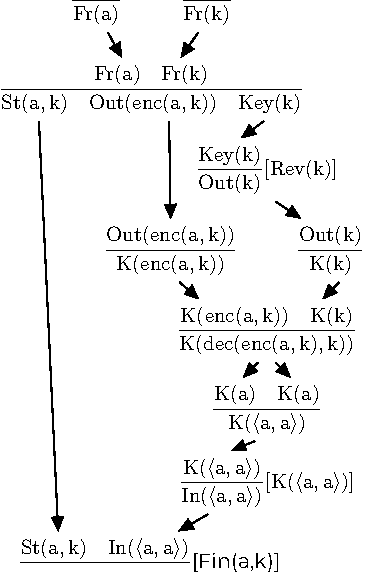
\includegraphics[width=.8\textwidth]
                    {./figures/lecture_4/dependency_graph_9}%
            \end{figure}
        \end{column}
    \end{columns}
\end{frame}

\begin{frame}[fragile]{Dependency graph definition}
    Let $E$ be an equational theory and $R$ be a set of multiset rewriting 
    rules. We say that $dg = (I, D)$ is a dependency graph modulo $E$ for $R$ 
    if $I \in (ginsts(R \cup \{\textsc{Fresh}\}))^{*}$, $D \subseteq \mathbb{N}
    ^2 \times \mathbb{N}^2$, and $dg$ satisfies the following conditions:

    \begin{table}
        \raggedright
        \begin{tabular}{ll}
            \textbf{DG1} & \multicolumn{1}{p{.85\textwidth}}{
                For every edge $(i, u) \rightarrowtail (j, v) \in D$, it holds 
                that $i < j$ and the conclusion fact of $(i, u)$ is equal 
                modulo $E$ to the premise fact of $(j, v)$.
            } \\
            \textbf{DG2} & \multicolumn{1}{p{.85\textwidth}}{
                Every premise of $dg$ has exactly one incoming edge.
            } \\
            \textbf{DG3} & \multicolumn{1}{p{.85\textwidth}}{
                Every linear conclusion of $dg$ has at most one outgoing edge.
            } \\
            \textbf{DG4} & \multicolumn{1}{p{.85\textwidth}}{
                The \textsc{Fresh} rule instances in $I$ are unique.
            }
        \end{tabular}
    \end{table}
\end{frame}

\begin{frame}[fragile]{Dependency graphs and traces}
    \begin{itemize}
        \item Dependency graphs provide us with an alternative formulation of 
              the multiset rewriting semantics given in the previous lectures
        \item We exploit this alternative semantic in our backwards 
              reachability analysis by incrementally constructing dependency 
              graphs instead of (action-)traces.
        \item Theorem: \textit{for every multiset rewriting system R and every 
              equational theory E, holds that:}
              \[traces_E (R) =_E {trace(dg)\;|\;dg \in dgraphs_E (R)}\]
    \end{itemize}
\end{frame}

\begin{frame}[fragile]{Finding traces}
    \begin{itemize}
        \item \textbf{Goal:} Derive constraints from the multiset rewriting 
              rules and properties to prove that \textit{at least one} possible 
              trace exists
        \item \textbf{Constraint solving} (intuition):
        \begin{enumerate}
            \item Create an empty constraint system
            \item Add node constraints corresponding to the actions in the 
                  formula
            \begin{itemize}
                \item e.g., not Ex A(x): add rules that contain A(x)
                \item If variables are used, consider them free
            \end{itemize}
            \item Add premise constraints for the nodes we added in the 
                  previous step
            \item Continue adding node and edge constraints (with equal 
                  variables) until we can construct a trace
        \end{enumerate}
    \end{itemize}
\end{frame}

\begin{frame}[fragile]{Dependency graph example}
    \begin{columns}
        \begin{column}{.6\textwidth}
            \begin{table}[]
                \footnotesize
                \raggedright
                {\setbeamercolor{alerted text}{fg=red}
                \begin{tabular}{lcl}
                    $PE$
                      & := &
                        $\left\{
                            \alert<3>{\dfrac{Fr(a)\quad Fr(k)}{St(a,k)\quad Out(enc(a,k))\quad Key(k)}}
                        \right\}$ \\[4mm]
                      & $\cup$ &
                        $\left\{
                            \alert<2>{\dfrac{St(a,k)\quad In(\langle a,a \rangle)}{}[Fin(a,k)]}
                        \right\}$ \\[4mm]
                      & $\cup$ &
                        $\left\{
                            \alert<9>{\dfrac{Key(k)}{Out(k)}[Rev(k)]}
                        \right\}$ \\[4mm]
                    $MD$
                      & := &
                        $\left\{
                            \alert<8,9>{\dfrac{Out(x)}{K(x)}},\quad
                            \alert<5>{\dfrac{K(x)}{In(x)}[K(x)]},\quad
                            \alert<0>{\dfrac{}{K(x:pub)}}
                        \right\}$ \\[4mm]
                      & $\cup$ &
                        $\left\{
                            \alert<0>{\dfrac{Fr(x:fresh)}{K(x:fresh)}{K (x:fresh)}}
                        \right\}$ \\[4mm]
                      & $\cup$ &
                        $\left\{
                            \alert<6,7>{\dfrac{K(x_1) \dots K(x_k)}{K(f(x_1 \dots x_k))}\;|\;f \in \sum^{k}}
                        \right\}$ \\[4mm]
                    $SR$
                      & := &
                        $\left\{
                            \alert<4>{\dfrac{}{Fr(x)}}
                        \right\}$
                \end{tabular}}
            \end{table}
        \end{column}
        \begin{column}{.4\textwidth}
            \begin{figure}
                \includegraphics<2>[width=.8\textwidth]{
                    ./figures/lecture_4/dependency_graph_1}%
                \includegraphics<3>[width=.8\textwidth]{
                    ./figures/lecture_4/dependency_graph_2}%
                \includegraphics<4>[width=.8\textwidth]{
                    ./figures/lecture_4/dependency_graph_3}%
                \includegraphics<5>[width=.8\textwidth]{
                    ./figures/lecture_4/dependency_graph_4}%
                \includegraphics<6>[width=.8\textwidth]{
                    ./figures/lecture_4/dependency_graph_5}%
                \includegraphics<7>[width=.8\textwidth]{
                    ./figures/lecture_4/dependency_graph_6}%
                \includegraphics<8>[width=.8\textwidth]{
                    ./figures/lecture_4/dependency_graph_7}%
                \includegraphics<9>[width=.8\textwidth]{
                    ./figures/lecture_4/dependency_graph_8}%
                \includegraphics<10>[width=.8\textwidth]{
                    ./figures/lecture_4/dependency_graph_9}
            \end{figure}
        \end{column}
    \end{columns}
\end{frame}

\begin{frame}[fragile]{Does this always work?}
    \begin{itemize}
        \item<2-> There is only one possible source for \texttt{St(a,k)}
        \item<3-> There is no rule that produces \texttt{Out($\langle
                  \mathrm{a,a} \rangle$)} so it must come from the attacker. 
                  \textbf{How did the attacker construct it?} Multiple options!
    \end{itemize}
    \begin{figure}
        \includegraphics<1>[width=.6\textwidth]
            {./figures/lecture_4/dependency_graph_alt_1}%
        \includegraphics<2>[width=.6\textwidth]
            {./figures/lecture_4/dependency_graph_alt_2}%
        \includegraphics<3>[width=.6\textwidth]
            {./figures/lecture_4/dependency_graph_alt_3}%
        \includegraphics<4>[width=.6\textwidth]
            {./figures/lecture_4/dependency_graph_alt_4}%
        \includegraphics<5>[width=.6\textwidth]
            {./figures/lecture_4/dependency_graph_alt_5}%
        \includegraphics<6>[width=.6\textwidth]
            {./figures/lecture_4/dependency_graph_alt_6}%
        \includegraphics<7>[width=.6\textwidth]
            {./figures/lecture_4/dependency_graph_alt_7}%
        \includegraphics<8>[width=.6\textwidth]
            {./figures/lecture_4/dependency_graph_alt_8}%
    \end{figure}
\end{frame}

% ---------------------------------------------------------------------------- %

\section{Constraint Systems}

% ---------------------------------------------------------------------------- %

\begin{frame}[fragile]{Construction and deconstruction}
    We need to prevent the attacker from performing \textbf{unnecessary} steps
    \begin{itemize}
        \item No need to first construct, then deconstruct
        \begin{itemize}
            \item e.g., attacker learns \texttt{m} and \texttt{k}, then applies 
                  \texttt{enc(m, k)}, then applies \texttt{dec(enc(m, k), k)}
        \end{itemize}
        \item For compound (non-atomic) terms, the attacker can either
        \begin{itemize}
            \item construct them, or
            \item learn them from an \texttt{Out()} fact
        \end{itemize}
        \item We can use this!
        \begin{itemize}
            \item When considering the possibility that a term was
                  deconstructed, there must be a \textbf{chain} from an 
                  \texttt{Out()} to the \texttt{K()} fact
        \end{itemize}
    \end{itemize}
\end{frame}

\begin{frame}[fragile]{Attacker deduction through (de)construction}
    \textbf{Construction rules:}\\[4mm]
        $\mathrm{\quad \dfrac{}{K^{\uparrow}(x:pub)}[K^{\uparrow}(x:pub)]}$
        $\mathrm{\quad \dfrac{Fr(x:fresh)}{K^{\uparrow}(x:fresh)}[K^{\uparrow}(x:fresh)]}$
        $\mathrm{\quad \dfrac{K^{\uparrow}(x)}{K^{\uparrow}(h(x))}[K^{\uparrow}(h(x))]}$\\[4mm]
        $\mathrm{\quad \dfrac{K^{\uparrow}(x)\quad K^{\uparrow}(y)}{K^{\uparrow}(enc(x,y))}[K^{\uparrow}(enc(x,y))]}$
        $\mathrm{\quad \dfrac{K^{\uparrow}(x)\quad K^{\uparrow}(y)}{K^{\uparrow}(dec(x,y))}[K^{\uparrow}(dec(x,y))]}$\\[4mm]
        $\mathrm{\quad \dfrac{K^{\uparrow}(x)\quad K^{\uparrow}(y)}{K^{\uparrow}(\langle x,y \rangle)}[K^{\uparrow}(\langle x,y \rangle)]}$
        $\mathrm{\quad \dfrac{K^{\uparrow}(x)}{K^{\uparrow}(fst(x))}[K^{\uparrow}(fst(x))]}$
        $\mathrm{\quad \dfrac{K^{\uparrow}(x)}{K^{\uparrow}(snd(x))}[K^{\uparrow}(snd(x))]}$\\[4mm]
    \textbf{Deconstruction rules:}\\[4mm]
        $\mathrm{\quad \dfrac{K^{\downarrow}(\langle x,y \rangle)}{K^{\downarrow}(x)}}$
        $\mathrm{\quad \dfrac{K^{\downarrow}(\langle x,y \rangle)}{K^{\downarrow}(y)}}$
        $\mathrm{\quad \dfrac{K^{\downarrow}(enc(x,y))\quad K^{\uparrow}(y)}{K^{\downarrow}(x)}}$\\[4mm]
\end{frame}

\begin{frame}[fragile]{Message deduction: (de)construction}
    \textbf{Communication rules:}\\[4mm]
        $\mathrm{\quad \textsc{Irecv}\dfrac{Out(x)}{K^{\downarrow}(x)}}$
        $\mathrm{\quad \textsc{Isend}\dfrac{K^{\uparrow}(x)}{In(x)}[K(x)]}$\\[4mm]
    \textbf{Coerce rule:}\\[4mm]
        $\mathrm{\quad \textsc{Coerce}\dfrac{K^{\downarrow}(x)}{K^{\uparrow}(x)}[K^{\uparrow}(x)]}$
\end{frame}

% ---------------------------------------------------------------------------- %

\section*{Summary}

% ---------------------------------------------------------------------------- %

\begin{frame}[fragile]{Summary}
    \begin{itemize}
        \item We now know how to model..
        \begin{itemize}
            \item ..protocol behavior as \textbf{multiset rewriting rules}
            \item ..protocol properties as \textbf{first-order logic formulas}
        \end{itemize}
        \item We also have an intuition of Tamarin's workflow and how to 
              represent the system as \textbf{dependency graphs}
        \item In the next lecture, we will talk more about constraint solving
    \end{itemize}
\end{frame}

% ---------------------------------------------------------------------------- %
% Reading Material
% ---------------------------------------------------------------------------- %
\begin{frame}[fragile]{Reading material}
    \textbf{Recommended reading}:
        ~\cite[Ch. 6--6.5]{tamarin-book},
        ~\cite{schmidt2012tamarin}
    \printbibliography[heading=none]
\end{frame}
% ---------------------------------------------------------------------------- %

\end{document}
